\subsubsection{Use Case}
Here follows the use case diagram: \\

\begin{figure}[H]
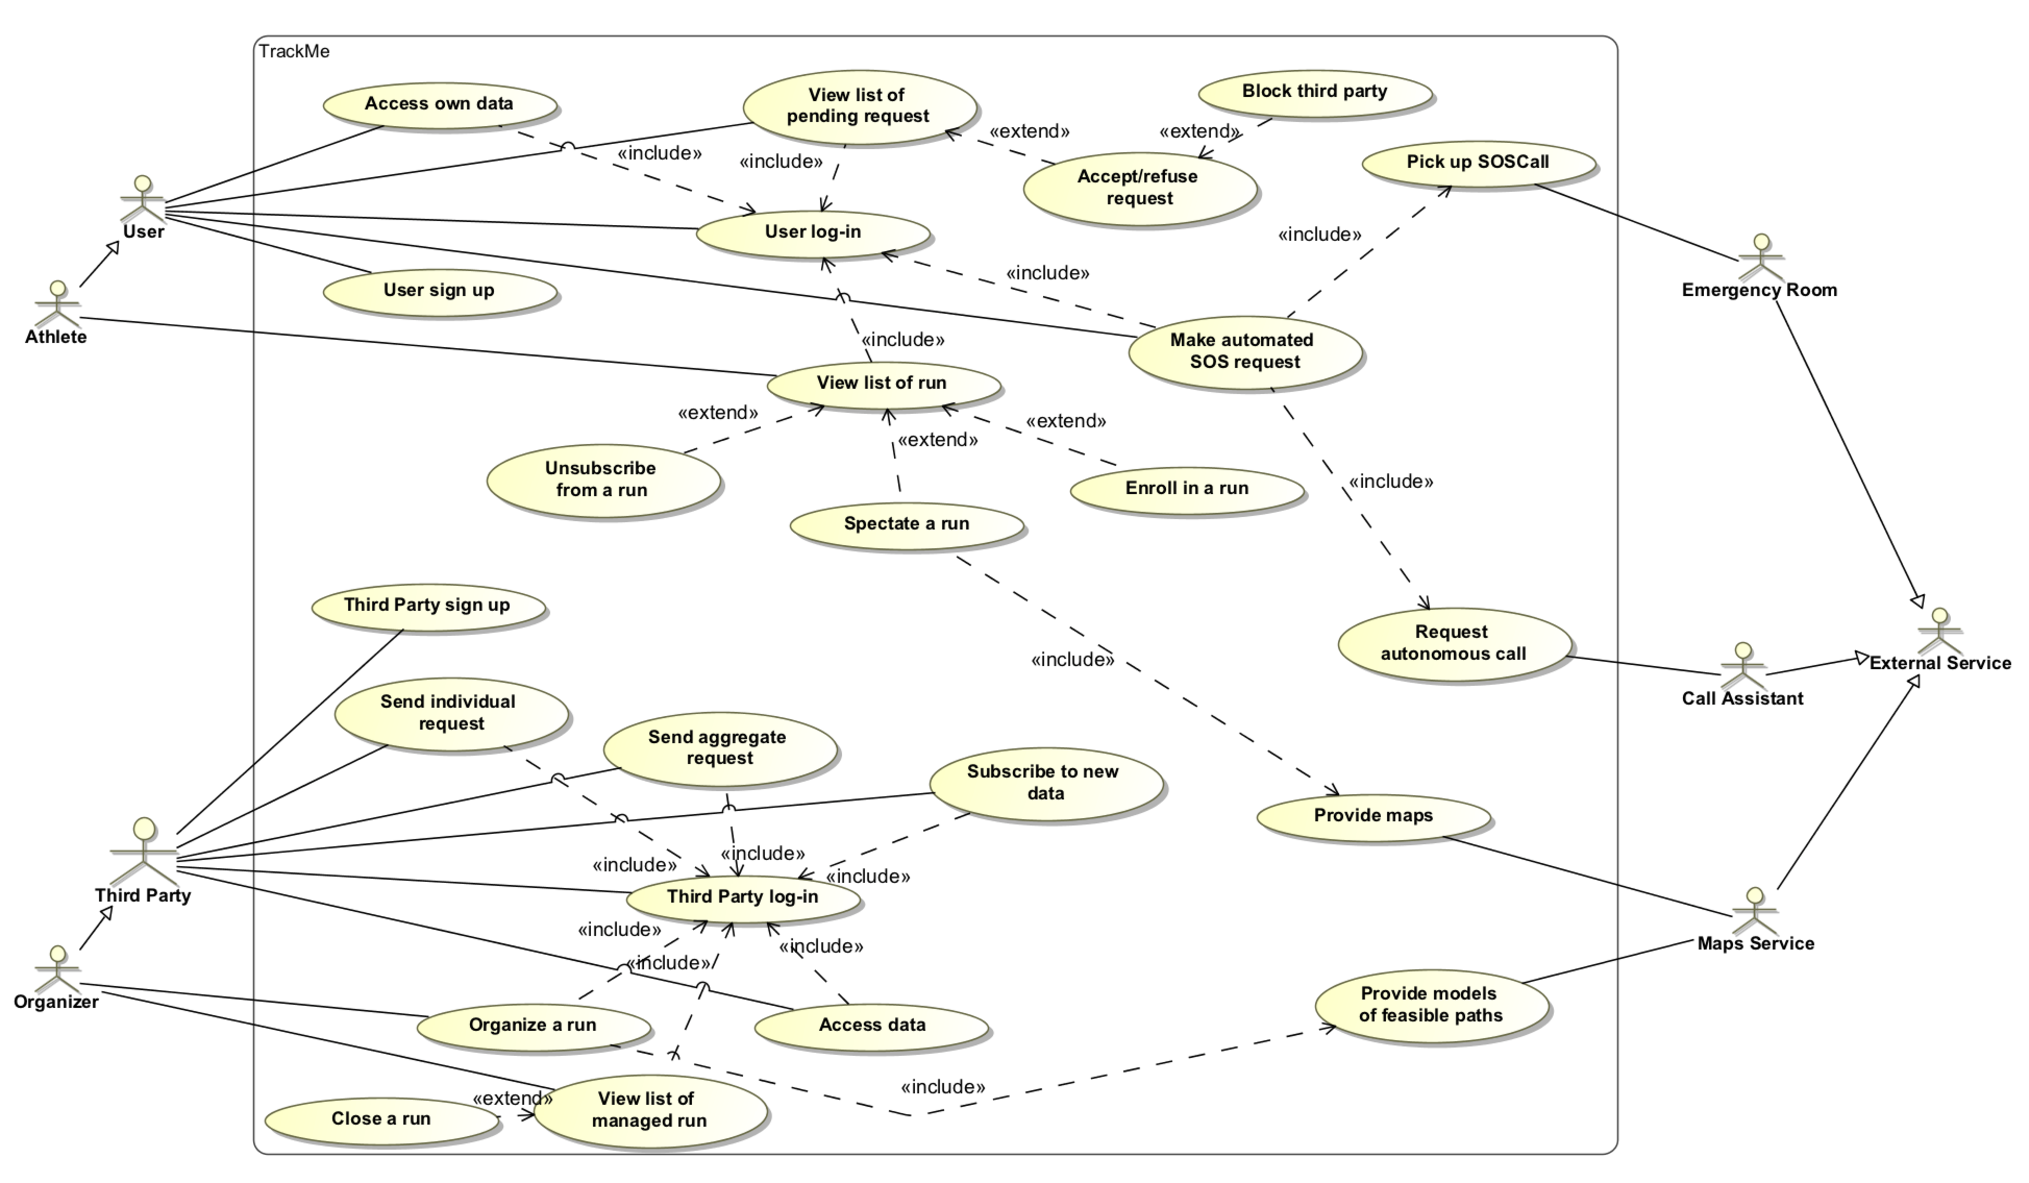
\includegraphics[width=\linewidth]{Images/usecase}
\caption{Use case diagram}
\label{fig:usecasediagram}
\end{figure}

\par 
Beneath, the use case are analyzed:	\\

\begin{table}[H]
\begin{tabularx}{\textwidth}{|l|X|}
\hline
 Name & Send aggregated request \\ \hline
 Actor & Third party customer  \\ \hline
 Entry conditions & Third party customer needs some aggregated data on anonymized users and the third party has performed log-in \\ \hline
 Event flow & 
 \begin{enumerate}
 	\item Third party customer compiles a form specifying the aggregated data that he wants to access
 	\item Third party customer sends the request
 	\item The system analyses the request and provides to the user the access to the data 
 \end{enumerate}   \\ \hline
 Exit conditions & The third party user can access the requested data \\ \hline
 Exceptions & If the request involves less or equal than 1000 distinct user, the access is not provided to the third party, that gets a notification \\ \hline
\end{tabularx}
\end{table}

\begin{table}[H]
\begin{tabularx}{\textwidth}{|l|X|}
\hline
 Name & Subscribe to new data \\ \hline
 Actor & Third party customer  \\ \hline
 Entry conditions & Third party customer needs some future aggregated data on anonymized users and the third party has performed log-in \\ \hline
 Event flow & 
 \begin{enumerate}
 	\item Third party customer compiles a form specifying the future aggregated data that he wants to access, when they will be available
 	\item Third party customer sends the request
 	\item The system waits for the moment in which all the future data requested will be generated 
 	\item The system analyses the request and provides to the user the access to the data 
 \end{enumerate}   \\ \hline
 Exit conditions & The third party user can access the requested data \\ \hline
 Exceptions & If the request involves less or equal than 1000 distinct user, the access is not provided to the third party, that gets a notification \\ \hline
\end{tabularx}
\end{table}

\begin{table}[H]
\begin{tabularx}{\textwidth}{|l|X|}
\hline
 Name & Organize run \\ \hline
 Actor & Third party customer \\ \hline
 Entry conditions & The third party customer has performed login and needs to organize a race\\ \hline
 Event flow & 
 \begin{enumerate}
 	\item The third party customer set up a run: he provides the name, the path, the date, the starting time, a closure date for the subscriptions and the minimum number of participants
  	\item The third party customer sends all the mentioned above information to the systme
 	\item The system adds the run to the list of the available races
 \end{enumerate}   \\ \hline
 Exit conditions & The race has been successfully added to the list of the available run \\ \hline
 Exceptions & 
 \begin{enumerate}
 	\item The name is already used by another run
 	\item Another run is already been specified for the same date and at least a portion of the path is overlapping 
 \end{enumerate}  
 All the exceptions are handled in the same way: the race is not added to the list and the third party user gets notified of the unsuccessful operation 
 \\ \hline
\end{tabularx}
\end{table}


\begin{table}[H]
\begin{tabularx}{\textwidth}{|l|X|}
\hline
 Name & Enroll in a run \\ \hline
 Actor & Athlete \\ \hline
 Entry conditions & The user wants to join to a run that has previously been added to the list of the available race \\ \hline
 Event flow & 
 \begin{enumerate}
 	\item The athlete accesses the list of available run
  	\item The athlete selects the race in which he wants to enroll
 	\item The athlete sends the request for joining the run to the system 
 	\item The system receives the requests and enroll the athlete in the race that he has specified 
 \end{enumerate}   \\ \hline
 Exit conditions & The athlete has been successfully enrolled to the race \\ \hline
 Exceptions &  
 \begin{enumerate}
 	\item The athlete is already enrolled to the race that he specifies in the request
 	\item The athlete is already been enrolled to a race in the same date of the run specified in the request 
 \end{enumerate}
 All the exceptions are handled in the same way: the athlete is notified that the enrollment was unsuccessful, by providing a brief motivation. Of course, the subscription process is aborted  
 \\ \hline
\end{tabularx}
\end{table}


\begin{table}[H]
\begin{tabularx}{\textwidth}{|l|X|}
\hline
 Name & Block requests from a company \\ \hline
 Actor & User \\ \hline
 Entry conditions & The user wants to block the request from a specific company \\ \hline
 Event flow & 
 \begin{enumerate}
 	\item The user accesses the list of available requests
  	\item The user selects the request which he wants to block
 	\item The user, with the express button, sends the request to TrackMe for classify as spam the selected request 
 	\item The system receives the requests and permanently blocks the company that sent the request.
 	\item The system notifies the user that the company is blocked
 \end{enumerate}   \\ \hline
 Exit conditions & The company had been successfully blocked \\ \hline
 Exceptions &  
 \begin{enumerate}
 	\item The company is already blocked.
 \end{enumerate}
 The exceptions are handled by the notification that the block of the company was unsuccessful, by providing a brief motivation.  
 \\ \hline
\end{tabularx}
\end{table}


\begin{table}[H]
\begin{tabularx}{\textwidth}{|l|X|}
\hline
 Name & Shared data with a third party\\ \hline
 Actor & User \\ \hline
 Entry conditions & The user wants to share data with a third party that it sent you a shared data request \\ \hline
 Event flow & 
 \begin{enumerate}
 	\item The user accesses the list of available requests
  	\item The user selects the request which he wants to accept
 	\item The user accept the request from a specific company
 	\item The system receives the acceptance and notifies both the third party and the user of the successful of the operation
 	\item The system provide the user health information to the third party
 \end{enumerate}   \\ \hline
 Exit conditions & The health status of the user is provided to the third party \\ \hline
 Exceptions &  
 \begin{enumerate}
 	\item The user accepts the request, but there are not available data in the system.
	\item The user accepts a request that has already accepted 
 \end{enumerate}
 The first exception is handle by notifying the third party that there are not available data stored in the system and it provides the data as soon as possible.
 The second exception is handle by notifying the user that the request has already accepted.
 \\ \hline
\end{tabularx}
\end{table}


\begin{table}[H]
\begin{tabularx}{\textwidth}{|l|X|}
\hline
 Name & Sign up \\ \hline
 Actor & User \\ \hline
 Entry conditions & The user wants to join to the application but he has not already registered \\ \hline
 Event flow & 
 \begin{enumerate}
 	\item The user click on the sign up button
  	\item The user complete the registration's form and provide his information
 	\item The user send the form to the system
 	\item The system checks that an account associated with identification information and social security number does not exists
 	\item The system notify to the user the success of the operation
 \end{enumerate}   \\ \hline
 Exit conditions & The user receive the notify about the successful of the operation \\ \hline
 Exceptions &  
 \begin{enumerate}
 	\item The user has already sign up into the application
 	\item The user doesn't provide valid data 
 	\item The username has already taken 
 \end{enumerate}
 The first exception is handle by notifying that the user has already subscribe into the application.
 All other exceptions are handled in the same way: the user is notified that the subscription was unsuccessful, by providing a brief motivation. The user is remanded to the sign up page.  
 \\ \hline
\end{tabularx}
\end{table}


\begin{table}[H]
\begin{tabularx}{\textwidth}{|l|X|}
\hline
 Name & Login \\ \hline
 Actor & User \\ \hline
 Entry conditions & The user wants to join into the application and he has already registered into the application\\ \hline
 Event flow & 
 \begin{enumerate}
 	\item The user enters his credentials in the “Username” and “Password” fields of the login page of “Data4Help” application 
  	\item The system checks the information provided by the user
 	\item The system redirects the user to the application home page
 \end{enumerate}   \\ \hline
 Exit conditions & The user is logged in the application \\ \hline
 Exceptions &  
 \begin{enumerate}
 	\item The user enters invalid username
 	\item The user enters invalid password 
 \end{enumerate}
 All the exceptions are handled in the same way: the user is notified that the logged in procedure was unsuccessful, by providing a brief motivation. Then the user is remanded to the login page.
 \\ \hline
\end{tabularx}
\end{table}